\parindent=0em
\subsection{Industria}
\noindent

%https://news.microsoft.com/es-es/2019/06/18/airbus-vuela-mas-alto-con-ayuda-de-la-tecnologia-de-realidad-mixta-de-microsoft/

%https://marquesme.com/5-beneficios-clave-de-realidad-mixta-para-la-industria/

%https://www.abc.es/tecnologia/informatica/soluciones/abci-realidad-mixta-y-hologramas-llegan-reuniones-trabajo-sector-inmobiliario-201903170153_noticia.html

Otro ámbito que es potenciado por la realidad mixta es la industria, esta tecnología beneficia a este sector de las siguientes formas:

\begin{itemize}
    \item \textbf{Proceso de control de calidad más rápido:} Estos largos procesos de control de calidad se ven reducidos notablemente haciendo uso de imágenes, textos o modelos 3D. Esto da lugar a ensamblajes más rápidos y con menos errores.
    
     \item \textbf{Mantenimientos más rápidos:} Se pueden sustituir manuales de reparación tediosos por simples instrucciones en el entorno de realidad mixta. Otro uso para agilizar el mantenimiento es el que hace, por ejemplo, la empresa de ascensores \textit{ThyssenKrupp} donde sus empleados, haciendo uso de estos cascos de realidad mixta, realizan llamadas al soporte técnico que les guía con facilidad gracias a poder superponer en tiempo real distintos elementos del ascensor a través de la retransmisión que ofrecen las gafas.
     
     \item \textbf{Reuniones colaborativas:} Los cascos de realidad mixta aportan utilidad de cara a trabajar de forma colaborativa mediante reuniones a distancia en tiempo real. Se crean hologramas de los participantes en un entorno concreto en el que pueden colaborar en diversos proyectos o participar de forma conjunta en lluvias de ideas.
     
\end{itemize}

 Todos los puntos anteriores fomentan el crecimiento de la empresa en forma de automatizar procesos, minimizar tiempos y reducir costes, es por esto que el uso de dicha tecnología es necesaria para ser competitivos.\\

La empresa de diseño, fabricación y venta de aviones civiles Airbus es una de las beneficiadas por la realidad mixta, esta empresa afirma que el uso de gafas de realidad mixta en su producción aumenta su productividad y su eficacia, además, utiliza estos HMD para formar a sus empleados (figura~\ref{fig:ingenierosAirbusHololens2}). Del mismo modo, aseguran que la tecnología \textit{hand tracking} de algunas de las gafas aporta seguridad a los empleados gracias a tener las manos libres. 

\begin{figure}[h]
    \centering
    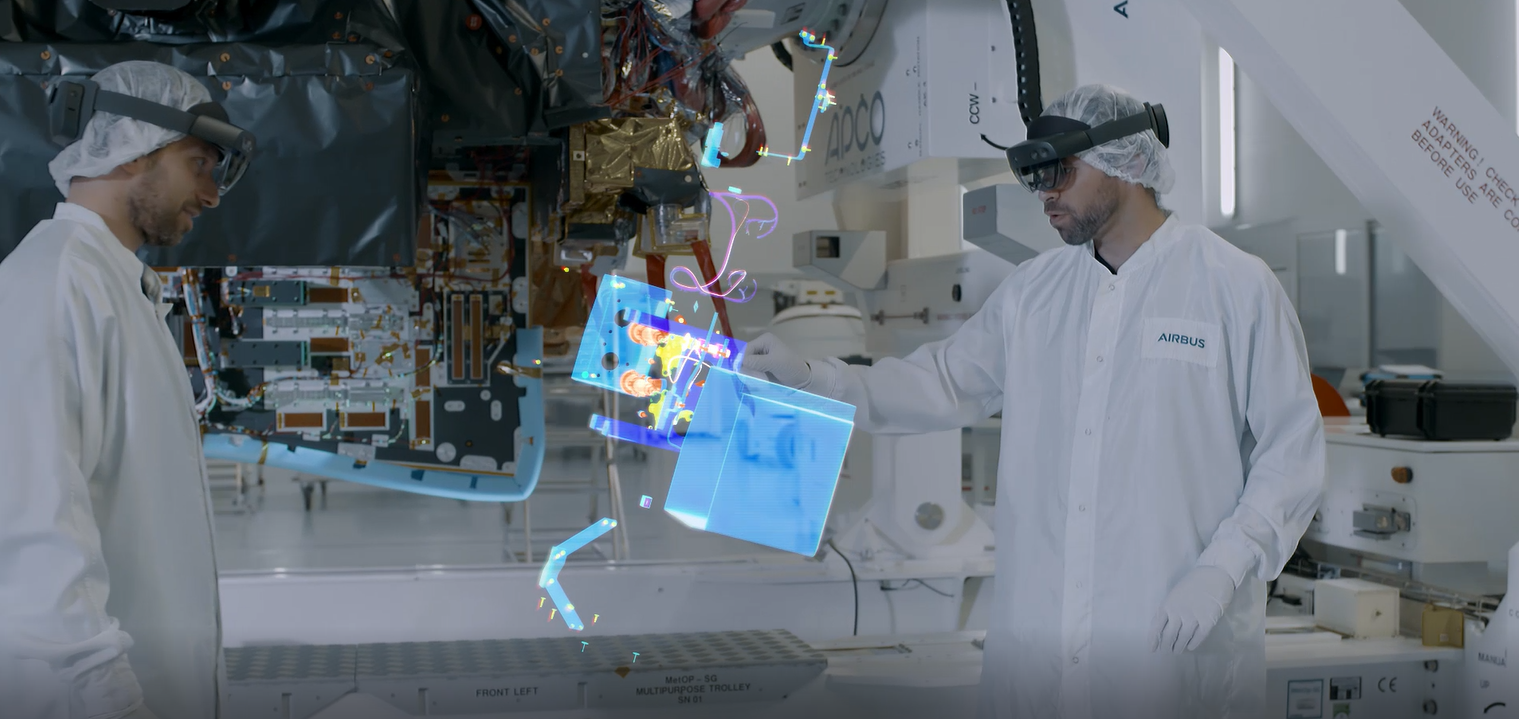
\includegraphics[scale=0.3]{Images/Estado del arte/ingenierosAirbus.png}
    \caption[Diseñadores de Airbus haciendo uso de la realidad mixta]{Diseñadores de Airbus haciendo uso de la realidad mixta\footnotemark.}
    \label{fig:ingenierosAirbusHololens2}
\end{figure}

\footnotetext{Fuente: \href{https://news.microsoft.com/es-es/2019/06/18/airbus-vuela-mas-alto-con-ayuda-de-la-tecnologia-de-realidad-mixta-de-microsoft/}{\nolinkurl{https://news.microsoft.com/es-es/2019/06/18/}}}

Por último, otro uso industrial de la realidad mixta es el que se puede aplicar al diseño de apariencia y estética de productos industriales como coches o motocicletas~\cite{mrinaesthethics}. En este caso, la aplicación \textit{Spacedesign} sustituye las técnicas de prototipado rápido por una experiencia de realidad mixta para realizar esos bocetos en tres dimensiones.
